\chapter{Results}
\section{Fixed coupling with pure pQCD interaction}
\begin{figure}
\centering
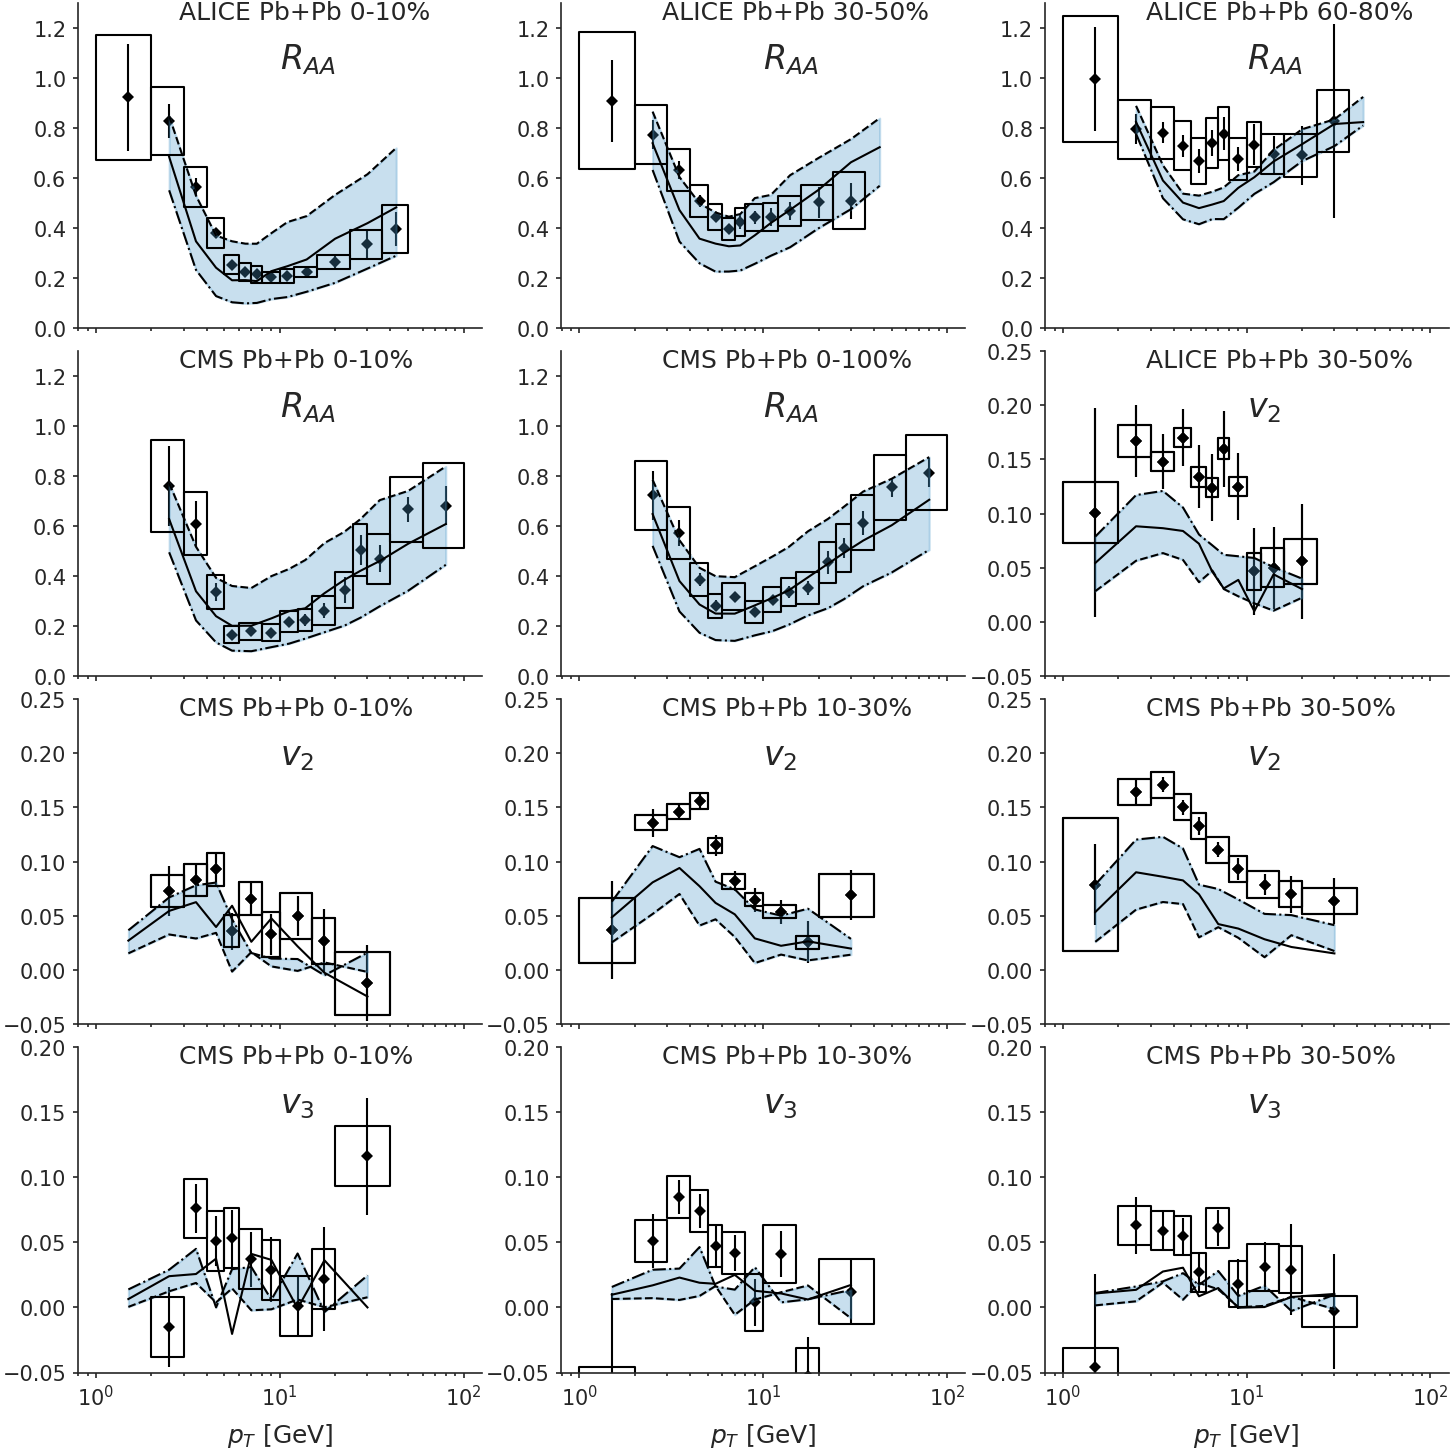
\includegraphics[width=\textwidth]{New-analysis/fix_alphas.png}
\caption{}
\label{fig:new:fix-a}
\end{figure}


\section{Calibration with a simpler implementation of the LPM effect}
\begin{center}
\begin{table}[h]
\caption{ALICE dataset}\label{table:ALICE-obs} 
\begin{tabularx}{\columnwidth}{XXX}
\hline 
 Observables & Centrality & Reference\\ 
\hline 
$D$-meson $v_2$ & 30-50\% & {Acharya:2017qps}\\ 
\hline 
Event-engineered $D$-meson $v_2$ & 30-50\% & {Grosa:2017zcz}\\ 
\hline 
$D$-meson $R_{AA}$ & 0-10, 30-50, 50-80\% & {Acharya:2018hre}\\
\hline 
\end{tabularx}
\end{table}
\begin{table}[h]
\caption{CMS dataset}\label{table:CMS-obs} 
\begin{tabularx}{\columnwidth}{XXX}
\hline 
Observables & Centrality & Reference\\ 
\hline 
D${}^0$-meson $v_2$ & 0-10, 10-30, 30-50\% & {Sirunyan:2017plt}\\ 
\hline 
D${}^0$-meson $R_{AA}$ & 0-10\%, 0-100\% & {Sirunyan:2017xss}\\ 
\hline 
B${}^{\pm}$-meson $R_{AA}$ & 0-100\% & {Sirunyan:2017oug}\\ 
\hline 
\end{tabularx}
\end{table}
\end{center}

The parameters of our model in the heavy-flavor sector are:
\begin{itemize}
\item[1.] $\tau_0$ the time at which heavy quark energy loss starts, varying between $0.1$ fm/$c$ to $1.0$ fm/$c$,
\item[2.] $\mu$, the medium energy scale ($\mu\pi T$) that appears in the running coupling constant of the scattering component, varying from $1/3$ to $4$,
\item[3.] $\kappa_D$, the strength of momentum diffusion at $ET = 1 \textrm{GeV}^2$, ranging from $0$ to $8$, and
\item[4.] $x_D$, the fraction of the momentum diffusion that is energy independent, ranging from $0$ to $1$.
\end{itemize}
In addition to these continuous parameters, the choice of different nuclear parton distribution functions acts as a discrete variable.

In this work, we sampled 80 design points in a four dimensional parameter space $(\tau_0, \mu, \kappa_D, x_D)$.
For each parameter set, we run 4000 minimum bias events.
Each event propagates an ensemble of $4\times 10^4$ charm quarks and $10^4$ bottom quarks.
The centrality is defined by the mid-rapidity charged particle multiplicity and the same kinematic cuts as are used by the experiments are applied to the calculation of heavy-flavor observables.
All observables are measured at 5.02 TeV in Pb+Pb, as listed in Table \ref{table:ALICE-obs} and \ref{table:CMS-obs}. Most of the data we utilize are for $D$-mesons: the
 $p_T$ dependent $D$-meson nuclear modification factor $R_{AA}$ and $p_T$ dependent second-order azimuthal anisotropy $v_2$ at various centralities {Sirunyan:2017plt, Sirunyan:2017xss, Acharya:2017qps,Grosa:2017zcz}.
We also compare to the event-shape-engineered $D$-meson $v_2$ measured by the  ALICE collaboration {Grosa:2017zcz}.
The idea of the event-shape engineering is to subdivide events at a certain centrality according to the magnitude of the charged particle $q$-vector, in this case,
\begin{eqnarray}
|q_2|^2 = \frac{\left(\sum_{i=1}^{M} \cos(2\phi) \right)^2+ \left(\sum_{i=1}^{M} \sin(2\phi) \right)^2}{M} \, .
\end{eqnarray}
The $D$-meson $v_2$ is measured for those events with $20\%$ highest $q_2$ and events with $60\%$ lowest $q_2$.
It is found that $D$-meson flow is strongly correlated with this measurement of bulk collectivity.
This event-shape-engineering procedure necessitates a full event-by-event study and may be sensitive to the interplay between heavy quark energy loss and initial condition fluctuations, so we include this observable into the set of observables on which we calibrate the model.
Finally in order to require the calibrated model to predict the desired mass-dependence, we include recent CMS measurements of $B^{\pm}$-meson $R_{AA}$, although the data have a large uncertainty which suppresses its importance in the likelihood function.
\begin{figure*}
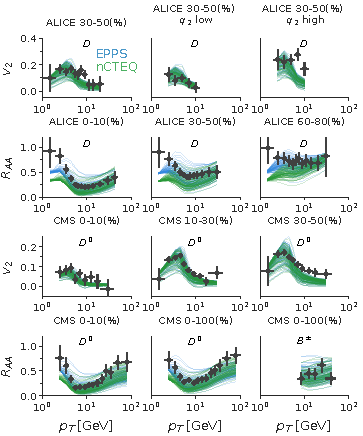
\includegraphics[width=.49\textwidth]{observables_design.pdf}
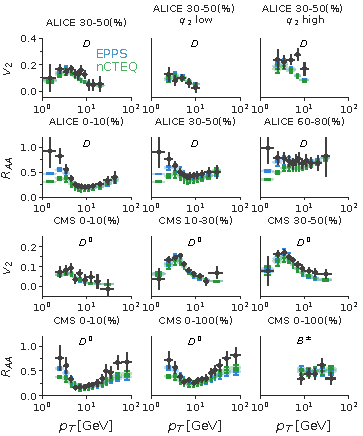
\includegraphics[width=.49\textwidth]{observables_posterior.pdf}
\caption{Left: the prior, i.e. the full range of calculations in parameter space. Right: the posterior, i.e. observables sampled from model emulators after calibration. In both figures, blue (green) lines are calculations with {\tt EPPS} ({\tt nCTEQ15np}) nuclear PDF.}\label{plots:deisgn_posterior_obs}
\end{figure*}

On the left of Figure \ref{plots:deisgn_posterior_obs}, we show the prior, i.e. the full range of our calculations in parameter space for each of the listed observables. 
We use different colors to distinguish calculations using {\tt EPPS} (blue) and
{\tt nCTEQnp} (green) nuclear PDF.
The calculated values of $R_{AA}$ at high transverse momenta and $v_2$ at low transverse momenta have a large spread, sufficiently wide to cover the experimental data.
We notice that the model always underestimates very low-$p_T$ $R_{AA}$ points and 30-50\% high-$p_T$ $v_2$ from CMS.
This could be a limitation of our model, such as the need of a more sophisticated implementation of the LPM effect or the need for a more accurate calculation of initial low-$p_T$ charm quark production in both $p$-$p$ and $A$-$A$ collisions. 
Plots on the right of Figure \ref{plots:deisgn_posterior_obs} show the posterior distribution of the observables from model emulators, i.e. interpolated model predictions after calibration.
The calibrated model displays a very good overall agreement with all the observables except for the cases pointed out above.
The use of different nuclear PDFs has a  negligible effect on azimuthal anisotropy observables, but does affect the $R_{AA}$ at small and large $p_T$.
Calculations with the {\tt EPPS} nuclear PDF work very well in describing $R_{AA}$ below $p_T = 50$ GeV, while calculations with the {\tt nCTEQnp} do slightly better for CMS $R_{AA}$ data with $p_T>50$ GeV.
The calculated event-engineered flow strongly correlates with the charged particle $|q_2|$ and describes the lowest 60\% $q_2$ bin very well.
For the highest 20\% $q_2$ bin, the model posterior is consistent with measurements below $5$ GeV and underestimates the data at higher $p_T$ bins.

\begin{figure}
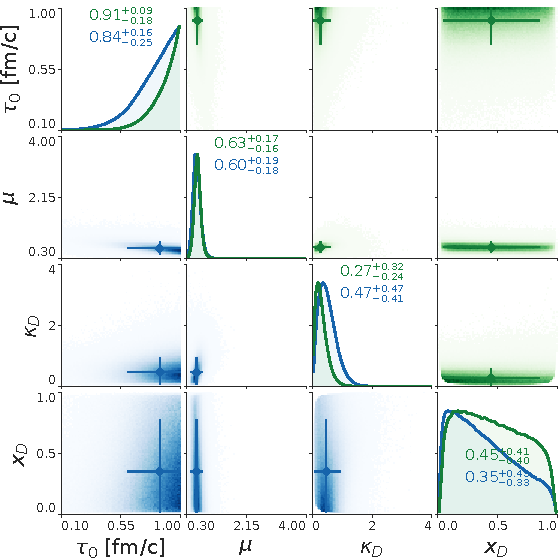
\includegraphics[width=.5\textwidth]{posterior.pdf}
\caption{Marginalized postrior probability distribution of model parameters. Diagonal plots show the marginalization on a single parameter. Off diagonal plots show the pair correlation between parameters. Blue (Geen) lines and lower (upper) off diagonal plots correspond to the extraction using EPPS (nCTEQ15np) nuclear PDF.}\label{plots:posterior}
\end{figure}
\begin{figure}
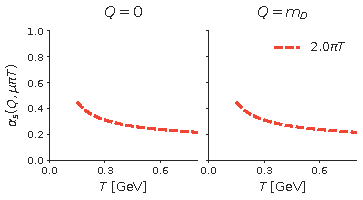
\includegraphics[width=.5\textwidth]{alpha_s_at_T.pdf}
\caption{Coupling constant with three values of the medium scale parameter $\mu$ taken  from the high likelihood region of the posterior. Left: $\alpha_s$ evaluated at a process scale $Q=0$. Right: $\alpha_s$ evaluated at a process scale $Q=m_D$.}\label{plots:alphas}
\end{figure}

The posterior probability distribution of all parameters is marginalized to single parameter distributions (diagonal) and two-parameter joint distributions (off-diagonal) in Figure \ref{plots:posterior}.
The lower off-diagonal plots and blue lines in the diagonal plots correspond to the calibration using the {\tt EPPS} nuclear PDF, and the upper off-diagonal plots and green lines in the diagonal plots use the {\tt nCTEQ15np} nuclear PDF.
Despite the difference in $R_{AA}$ when different nuclear PDFs are used, the extracted probability densities of parameters are similar.
To describe LHC data, the model prefers a late onset of medium induced energy loss and a medium energy scale roughly around $0.6\pi T$, which implies the largest coupling constant at a given temperature is $\alpha_s \sim \alpha_s(1.8T)$.
A small but finite amount of momentum diffusion at $ET=1\textrm{ GeV}^2$ is preferred for the diffusion component.
The smallness of this number is expected since most of the interaction is already taken account by the pQCD scattering component with a relatively large coupling constant (i.e. a small medium scale).
We find this study to be not sensitive to the energy / temperature dependence of the diffusion component beyond the regular $T^3$ scaling of the momentum diffusion constant.   

The preferred medium scale parameter $\mu \sim 0.6$ is not large which could result in a large $\alpha_s$.
Therefore, we check the range of typical $\alpha_s$ values in the model in order to evaluate the use of perturbative matrix-elements.
Figure \ref{plots:alphas} shows the coupling constant evaluated at two process scales $Q=0$ and $Q=m_D$.
In the case of $Q=0$ (left), the energy scale is cut off by $\mu\pi T$ and this plot show the maximum of model coupling constant at a given temperature.
Setting $Q=m_D$ (right) as a proxy for the typical momentum transfer in the $t-$channel scattering, the coupling constant rises slower as temperature drops.
It is found that in order to describe experimental data, the preferred coupling constant is fairly large, suggesting next-to-leading (NLO) order corrections to the present scattering picture should be prominent. 
Because these large $\alpha_s$ values are encountered in small-momentum-transfer scatterings ($0< Q < m_D$), we will absorb these small-momentum-transfer elastic and inelastic pQCD processes into a radiation-improved Langevin equation in future studies. 
This way, one not only avoids the explicit use of large $\alpha_s$ in pQCD matrix-elements, but also interpolates between the pQCD based scattering model, the radiation-improved Langevin model and pure non-perturbation drag and diffusion model with one or two control parameters, allowing for more systematic model-uncertainty study.

Next, we investigate the transport coefficients extracted from the calibrated model.
To define the transport coefficient of a heavy quark,
we combine the contribution from both elastic scatterings and the diffusion component,
\begin{eqnarray}\label{eq:qhat}
\frac{\hat{q}}{T^3} &=& \frac{1}{T^3}\frac{d}{dt}\left\langle p_\perp^2 \right\rangle\\
\nonumber
 &=&  \kappa_D\left(x_D + (1-x_D)\frac{\textrm{GeV}^2}{ET}\right) + \frac{\hat{q}_{\textrm{el}}}{T^3}.
\end{eqnarray}
Where $\hat{q}_{\textrm{el}}$ is obtained by integrating the rate equation with inserting the transverse momentum transfer square.
We shall discuss the inclusion of inelastic process into the calculation of $\hat{q}$ in section \ref{section:conclusion}.
Performing this calculation for many random parameter set samples drawn from the posterior distribution using either nuclear PDF, we determine the posterior distribution of the functional $\hat{q}(E, T)$ constrained by data.
On the left of Figure \ref{plots:posterior_qhat}, we showed the 95\% credible region of $\hat{q}$ as function of temperature, fixing the heavy quark momentum at $10$ GeV.
The right panel of the figure shows $\hat{q}$ as function of momentum at $T=0.35$ GeV.
Our formula includes a mass dependence -- therefore  the charm quark $\hat{q}$ (region enclosed by thick red lines and slashes) is slightly different from the bottom quark $\hat{q}$ (region enclosed by thick blue lines).
The present result is consistent with previous work by Xu et al (shaded region) {Xu:2017obm}, who used an improved Langevin model to extract the charm quark transport properties at the LHC,  but hits the lower half of the 95\% credible region of the previous extraction.
\begin{figure}
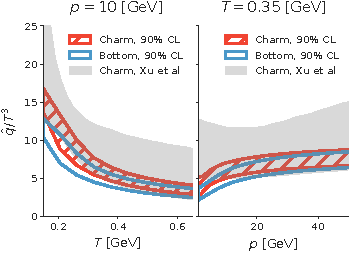
\includegraphics[width=\columnwidth]{qhat_p_T.pdf}
\caption{Posterior range of the heavy quark transverse momentum broadening parameter $\hat{q}$ from Equation \ref{eq:qhat}. The results include the uncertainty from using different nuclear PDFs. Blue boxed region is for bottom quarks and red slashed region for charm quarks. The shaded region indicates a previous extraction {Xu:2017obm}.}\label{plots:posterior_qhat}
\end{figure}
Alternatively, one can present our results in terms of the heavy quark spatial diffusion constant $D_s$ often defined in the limit of $p\ll M$.
It is related to the momentum diffusion parameter by
\begin{eqnarray}
2\pi T D_s = \frac{8\pi T^3}{\hat{q}(p\rightarrow 0, T)} \, .
\end{eqnarray}
In figure \ref{plots:posterior_Ds}, we plot the 95\% credible region of both the charm (region enclosed by red thick lines and slashes) and bottom (region enclosed by blue tick lines) quark spatial diffusion constant as function of $T/T_c$.
The results of this work is systematically higher than the extraction from the former work (shaded region).
There have also been attempts made to calculate the spatial diffusion constant of heavy quarks using lattice QCD: three calculations are available, two are calculated in the static heavy quark limit (blue and black symbols with higher values) {Banerjee:2011ra, Banerjee:2011ra}, one of which performs continuum extrapolation (black square) {Francis:2015daa}; the other result uses a realistic charm quark mass (red triangle symbols with lower values) {Ding:2012sp}.
Our posterior of $D_s$ including the diffusion contribution but with only elastic scattering agrees with the lattice evaluation in the static heavy quark limit.
The effect of including the inelastic scattering in $D_s$ will be discussed in the last section.

To summarize this section, we have performed a Bayesian calibration on the model parameters, yielding
generally good agreement to the data.
Although the use of different nuclear shadowing parametrizations does affect the shape of $R_{AA}$, the extracted parameters are not strongly affected.
The extracted parameters indicate a late onset of medium induced heavy quark energy loss and prefer a small but finite diffusion component.
The transport coefficient $\hat{q}$ and spatial diffusion constant $D_s$ are extracted with $D_s$ being compatible with lattice calculations in the static heavy quark limit. 

\begin{figure}
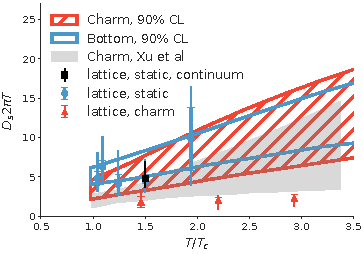
\includegraphics[width=\columnwidth]{Ds_posterior.pdf}
\caption{Posterior range of the heavy quark spatial diffusion coefficient. The blue boxed region is for bottom quarks and the red slashed region for charm quarks. The shaded region indicates a previous extraction in {Xu:2017obm}. Square and dimond symbols are lattice calculations in the static heavy quark limit {Banerjee:2011ra, Francis:2015daa}; triangular symbols are lattice calculations with physical charm quark mass {Ding:2012sp}.}\label{plots:posterior_Ds}
\end{figure}

We now apply the calibrated model to predict observables that have already been measured but were excluded in the calibration (validation) and also predict new observables.
In principal, any parameter set sampled according to the posterior probability distribution in the high-likelihood region (95\% credible for example) is equally good to make predictions and the resultant differences represent the systematic uncertainties of the calculation.
For simplicity, we only run a single set of high likelihood parameters listed in Table \ref{table:high-likelihood-parameters} for a large number of events.
\begin{table}
\caption{A high-likelihood parameter set}\label{table:high-likelihood-parameters}
\begin{tabularx}{\columnwidth}{XXXXX}
\hline
Parameters & $\tau_0$ [fm/$c$] & $\mu$ & $\kappa_D$ & $x_D$   \\
\hline
Values & 0.9 & 0.6 & 0.4 & 0.5\\
\hline
\end{tabularx}
\end{table} 
\begin{figure*}
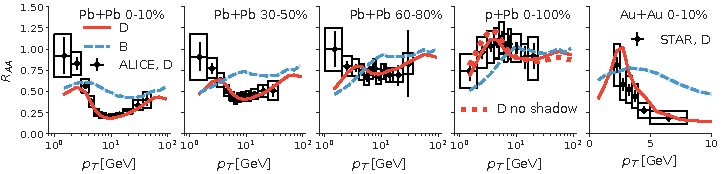
\includegraphics[width=\textwidth]{raa.pdf}
\caption{Calculation of heavy-flavor $R_{AA}$ using a high likelihood parameter set. Results are compared to ALICE $D$-meson measurements in Pb+Pb and p+Pb {Abelev:2014hha,Abelev:2014hha} and STAR $D$-meson measurements in Au+Au {Xie:2016iwq}. $B$-meson $R_{AA}$ are predicted.}\label{plots:pred:raa}
\end{figure*}
\begin{figure*}
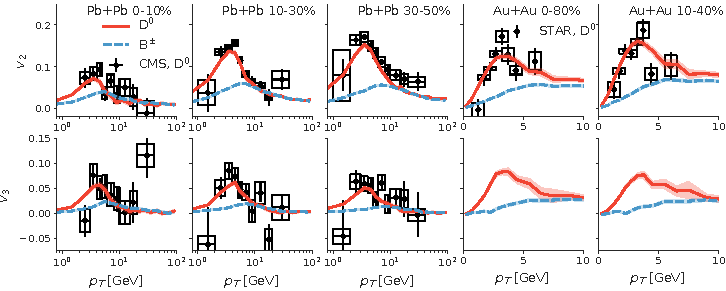
\includegraphics[width=\textwidth]{vn.pdf}
\caption{Calculation of heavy-flavor flows with a high likelihood parameter set. Results are compared to CMS $D$-meson measurements in Pb+Pb {Sirunyan:2017plt} and STAR $D$-meson measurements in Au+Au {Adamczyk:2017xur}. $D$-meson $v_3$ and $B$-meson $v_2, v_3$ are predictions.}\label{plots:pred:vn}
\end{figure*}
\begin{figure}
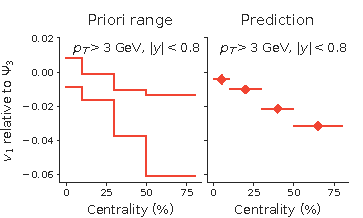
\includegraphics[width=0.5\textwidth]{v1.pdf}\\
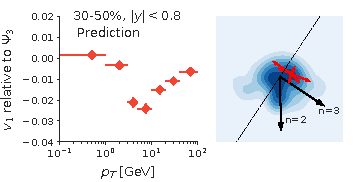
\includegraphics[width=0.5\textwidth]{v1pT.pdf}
\caption{Top row: centrality dependence of $D$-meson direct flow with respect to the $n=3$ event plane. Left: the prior range. Right: predictions using a high likelihood parameter set. Bottom left: the transverse momentum dependence of $D$-meson direct flow with respect to the $n=3$ event plane in the 30-50\% centrality bin. Bottom right: a sample TRENTo event. The third order eccentricity would drive a $v_3$. A measurement along the $n=3$ direction would introduce reflection asymmetry in the heavy quark energy loss.}\label{plots:pred:v1}
\end{figure}
We first study the nuclear modification factor in a larger range of $p_T$:
In Figure \ref{plots:pred:raa} the $D$-meson and $B$-meson $R_{AA}$ for 0-10\%, 30-50\%, and 60-80\% centrality are shown and compared to ALICE $D$-meson measurements.
The mass effect clearly separates $B$-meson from $D$-meson $R_{AA}$ in the intermediate $p_T$ range. 
The calculation for $p$+Pb collisions is shown in the fourth plot compared to ALICE measurements {Abelev:2014hha}.
The red-dotted line shows the calculation without nuclear shadowing for $p$+Pb collision.
We find that the calibrated model results are in a very good agreement with the description of the $p+Pb$ minimum bias measurement and that shadowing  is important to understand the low-$p_T$ data.
In the right most plot, we apply the model to Au+Au collisions at RHIC  ($\sqrt{s} = 200$ GeV).
The calculated $D$-meson $R_{AA}$ is slightly higher than the STAR measurement {Xie:2016iwq}, 
yet given that we did not include any RHIC data in our calibration, this level of agreement is satisfactory.

Next, we validate the calibrated model by comparing to CMS measured $D$-meson $v_3$ and make a prediction for $B$-meson $v_n$ in the first three columns of Figure \ref{plots:pred:vn}.
In the transport model, non-zero heavy-flavor $v_3$ is caused by heavy quarks losing energy to a medium that contains a third order eccentricity from initial condition fluctuations.
The $B$-meson $v_2$ and $v_3$ is predicted to be similar to $D$-meson flow for $p_T > 10$ GeV, below which $B$-meson flow is significantly smaller than $D$-meson flow.
Compared to CMS data, the calibrated model reproduces the transverse momentum and centrality dependence of $D$-meson $v_3$ very well.
In the last two columns of Figure \ref{plots:pred:vn}, we again apply the model to the RHIC data and observe a good agreement with STAR measured $v_2$ of $D^0$-mesons {Adamczyk:2017xur}.

Finally, we investigate $D$-meson direct flow $v_1$.
$D$-meson $v_1$ is tiny if one measures it with respect to the reaction plane due to the reflection symmetry on averaging over multiple events.
However, correlating heavy quark $v_1$ with charged particle $v_3$ results in a non-zero signal even at mid-rapidity.
This directed flow with respect to the $n=3$ event plane is calculated in the scalar product approach
\begin{eqnarray}
v_1 &=& \left\langle \frac{\Re\{q_3 Q_1^*\}}{mM} \right\rangle\Bigm/\sqrt{\left\langle \frac{|q_3|^2-m}{m(m-1)} \right\rangle}, \nonumber\\
Q_1 &=& \sum_{j=1}^{M}e^{i\phi_j} \textrm{, for heavy mesons},\nonumber\\
q_3 &=& \sum_{j=1}^{m}e^{i3\phi_j} \textrm{, for charged particles}. 
\end{eqnarray}
The resulting $v_1$ as function of centrality is shown in Figure \ref{plots:pred:v1}.
The upper left plot shows the prior range of this quantity as function of centrality using events from the 80 design points parameter set calculations.
The upper right dots are our prediction using the selected high likelihood parameter set.
The calculated $v_1$ is clearly finite and negative in our calculation and we expect it to reach as far as $-3\%$ in the peripheral centrality bin.
The transverse momentum dependence of $v_1$ is shown in the lower left plot, the magnitude of the signal grows with $p_T$ until it reaches the minimum at $p_T \sim 8$ GeV; then the magnitude slowly drop to zero at large $p_T$.
We understand this finite $v_1$ in the following way
(see also the sketch in the lower right of Figure \ref{plots:pred:v1}):
when $q_3$ is finite, the direction of $q_3$ defines a plane to which the medium evolution is reflection asymmetric and this asymmetry causes heavy quarks to loose energy differently depending on the direction of motion being along or against the direction of $q_3$.
Since $q_3$ originates from triangular initial state fluctuations, a finite signal would be another indication of heavy quark energy loss coupling to initial condition fluctuations and bulk collectivity.

\begin{figure}
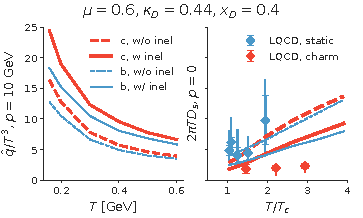
\includegraphics[width=0.5\textwidth]{qhat_full.pdf}
\caption{Comparison of the heavy quark transport coefficient (left: $\hat{q}$, right $D_s$) with (solid lines) and without (dashed lines) the inclusion of the inelastic contribution. Thin blue lines denote the bottom quark and thick red lines denote the charm quark region. Blue symbols are lattice calculations in static heavy quark limit {Banerjee:2011ra} and red symbols are lattice calculations with physical charm quark mass {Ding:2012sp}.}\label{plots:transport_full}
\end{figure}
Before summarizing this work, we want to return to the definition of $\hat{q}$ in our model.
In Equation (\ref{eq:qhat}), we  only included the elastic scattering processes in the second term and did not include inelastic scattering contributions to momentum broadening.
This is due to having an order-by-order definition of $\hat{q}$ in pQCD.
In fact, the inelastic scattering processes also contain a diffusion-like part, but this contribution is shown to be one order higher in $\alpha_s$ {Ghiglieri:2015ala}, though it may not be numerically small in a realistic scenario compared to leading order.
Since it was our goal to determine a leading order transport coefficient we justify the use of Equation (\ref{eq:qhat}) and neglect any contributions that can be attributed to higher order corrections. 
This choice is also conceptually cleaner for a comparison with other pQCD based calculations.
For lattice calculations the results do not rely on an expansion in $\alpha_s$.
In that case, in order to make a reasonable comparison with lattice transport coefficients, we should calculate $\hat{q}$ from the calibrated model including the inelastic scattering processes.
Unfortunately, currently there is no lattice calculation of $\hat{q}$ available at finite heavy quark momentum.  
$D_s$ on Lattice does exist, but the appropriate momenta ($p \ll M$) are too small for our calculation with Gunion-Bertsch matrix-elements to be valid.
Even so, we would like to show the $\hat{q}$ and $D_s$ with a set of high likelihood parameters that include the inelastic contribution.
Just as the energy loss shown in Figure \ref{plots:dEE}, the transverse momentum broadening per unit time in the presence of inelastic collision processes is not constant for a thin medium.
Therefore, we set up a Monte Carlo simulation for heavy quarks at fixed energy  and extract $\hat{q}$ only after the finite path length effect fades away. 
Figure \ref{plots:transport_full} compares the $\hat{q}$ at $p=10$ GeV and $D_s$ with and without inelastic collision channels.
The calculation uses the high likelihood parameter set in Table \ref{table:high-likelihood-parameters}. 
We observe a 30-40\% increase in $\hat{q}$ and similar amount of decrease in $D_s$ if the inelastic contributions are included.

To summarize, we have developed a novel linearized hybrid transport model, called {\tt Lido}, for heavy quark propagation inside a quark-gluon plasma.
Heavy quarks undergo perturbative scatterings with medium particles. Between subsequent scatterings, the propagation is driven by Langevin dynamics with empirical drag and diffusion coefficients.
Model parameters are calibrated using a Bayesian model-to-data analysis by comparing to $D$-meson and $B$-meson observables in Pb+Pb collisions at $\sqrt{s}=5.02$ TeV.
Our results suggest a late onset of medium energy loss.
The diffusion component to the overall transport coefficients is small, with the dominant contribution coming from the explicitly treated scattering processes.

The calibrated model predicts the centrality and $p_T$ dependence of the $B$-meson nuclear modification factor and flows and a non-zero $D$-meson direct flow with respect to $n=3$ event plane.
The extracted heavy quark transport coefficient $\hat{q}$ at finite momenta in the QGP phase is consistent within uncertainties with previous calibrations using an improved Langevin approach as well as with lattice QCD calculations.

\section{Comparison with the improved Langevin model calibration}

\section{Calibration with a more sophisticated transport model}
Finally, we apply the LIDO model to the extraction of the heavy quark transport coefficients.
In this analysis, the aspects we want to improve is that 
\begin{itemize}
\item A more sophisticated implementation of the LPM effect to reduce modeling uncertainty of the radiative process.
\item An interpolation of the diffusion picture and the scattering picture to take into account modeling uncertainty and an easy parametrization of the non-perturbative effect.
\item A better treatment of the interfacing between the high-virtuality evolution and the low-virtuality transport equation.
\end{itemize}
How we improve on each of these aspects has been elaborated in details in section [] and section [].

\paragraph{Model parameters}
Again we first describe the parameters and their prior range in table \ref{table:new:prior}
\begin{itemize}
\item[1] A medium scale parameter $\mu$ in the effect coupling that cuts off the running of $\alpha_s$ below the scale $\mu\pi T$, $\alpha_s(Q) = \frac{2\pi}{9}\left(\ln\frac{\max\{Q, \mu\pi T\}}{\Lambda_{\textrm{QCD}}}\right)^{-1}$.
\item[2] The energy loss starting time $\tau_i$.
\item[3] A matching scale parameter $R_v$ between the vacuum-like and medium-induced radiation $Q_{\textrm{sw}}^2 = R_v\Delta k_\perp^2$, where $\Delta k_\perp^2$ is the transverse momentum a vacuum branching could acquire from its in-medium transport.
\item[4] The switch scale parameter $c$ of momentum transfer between the scattering dynamics and the diffusion dynamics $Q_{\textrm{cut}}^2 = c m_D^2$.
\item[5-9] These five numbers $K,a,b,p,q$ parametrizes a correction, whose origin can be either perturbative or non-perturbative, to the leading order transport coefficient,
\begin{eqnarray}
\Delta\hat{q} &=& \frac{K T^3}{\left[1+\left(a\frac{T}{T_c}\right)^p\right]\left[1+\left(b\frac{E}{T}\right)^q\right]}
\end{eqnarray}
$K$ is the overall magnitude of the correction. $a$ and $p$ parametrize an deviation from the $T^3$ scaling of the $\hat{q}$ near $T_c$, while $b$ and $q$ parametrize the energy dependence.
\item[10] Finally, a $\gamma$ parameter relates the correction to the longitudinal transport parameter to the transverse one.
\begin{eqnarray}
\Delta\hat{q}_L &=& \frac{\Delta\hat{q}}{2} \left(\frac{E}{M}\right)^{\gamma}.
\end{eqnarray}
Note that such a construction goes back to an isotropic diffusion when velocity approaches zero ($E\rightarrow M$).
\end{itemize}

\begin{table}
\centering
\caption{Prior range of parameters}\label{table:new:prior}
\begin{tabular}{ccc}
Symbol & Description & Range \\
\hline
$\xi = \frac{\tau_i}{\tau_0}$ & energy loss starting time & (.1, .9) \\
$c = \frac{Q_{\textrm{cut}}^2}{m_D^2}$ & soft/hard switching scale & $(.1, 10.)$ \\
$R_v = \frac{Q_{\textrm{sw}}^2}{\Delta k_\perp^2}$ & vac/medium-ind. switching scale & $(0.14, \infty)$\\
$\mu$ & Running $\alpha_s$ stops at $Q = \mu\pi T$ & $(.6, 10)$ \\
$K$ & Norm for $\Delta \hat{q}$ & $(0, 20)$\\ 
$p$ & Additional $T$-dep power  & $(-2, 2)$\\ 
$q$ & Additional $E$-dep power  & $(-1, 1)$\\ 
$a$ & Additional $T$-dep scale  & $(-.5, 3)$\\ 
$b$ & Additional $E$-dep scale  & $(-.5, 3)$\\ 
$\gamma$ & Relation of $\Delta \hat{q}$ and $\Delta \hat{q}_L$  & (-1, 1)\\ 
\end{tabular}
\end{table}

We sampled 250 design points and 50 validation points. 
As a remark, we chosoe to give $c, R_v, \mu, a$ and $b$ an uniform prior in their $\log$ space.
This means that if we transform them back to the original space, the prior distribution will not be flat.
The reason we did these is because these parameters either causes a logarithmic slow change in the model or its prior uncertainty is large that it can be vary by orders of magnitude.
For example, the $\mu$ parameter enters the logarithmic running of $\alpha_s$ and we can rewrite the maximum possible $\alpha_s$ as,
\begin{eqnarray}
\alpha_{s,\max}(T) = \frac{2\pi}{9}\frac{1}{\ln(\mu) + \ln(\pi T/\Lambda_{\textrm{QCD}})}
\end{eqnarray}
Therefore, we choose assign a uniform prior to $\ln(\mu)$ so that $\alpha_s$ also varies notable within the prior range.
As for the $c$ parameter, it controls the boundary of the scattering and diffusion approximation, within a reasonable range of $c$, the diffusion dynamics and the scattering dynamics results in a similar amount of energy loss as has been shown in section [], and difference is seen in more subtle observables, therefore it is also assumed to be flat in the $\log$ space.
For $R_v, a$ and $b$, we did this to allow an order of magnitude change in the parameters as we want to test both the large and small number limits.

\begin{figure}
\centering
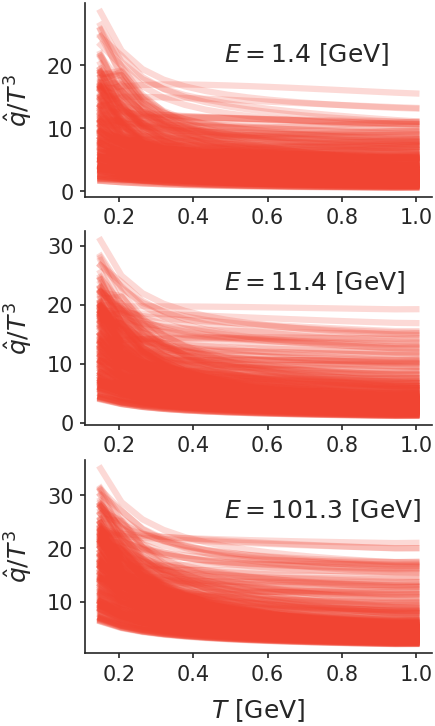
\includegraphics[width=.4\textwidth]{New-analysis/qhat_prior.png}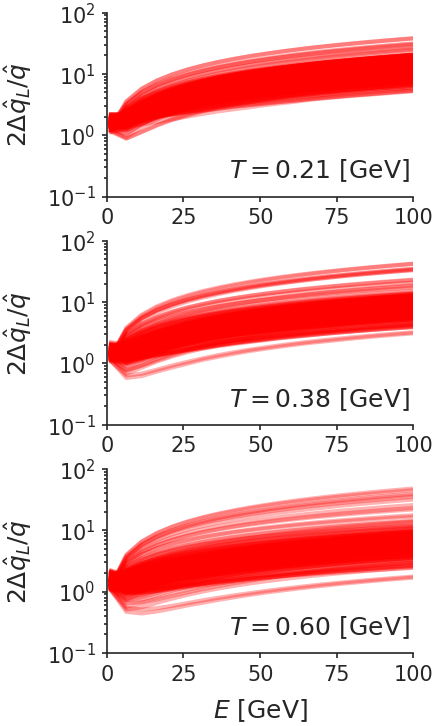
\includegraphics[width=.4\textwidth]{New-analysis/ER_prior.png}
\caption{•}
\label{fig:new:design-qhat}
\end{figure}

To get an idea of what the prior range of the transport parameters looks like, we combine those parameters that enters the computation of the total $\hat{q}$ (including scattering, perturbative diffusion and parametrized correction contribution) and plot them as function of temperature and energy in figure \ref{fig:new:design-qhat}. 
On the left, 250 design's $\hat{q}$ as function of temperatures are shown. Each subplots corresponds to a charm quark energy of $1.4$ GeV, $11.4$ GeV and $101.3$ GeV.
The prior range of $\hat{q}$ varies over a order of magnitude.
On the right of the figure, we show the ratio between the two times of the total $\hat{q}_L$ and $\hat{q}$, if the transport parameters are isotropic, this ratio should be unity.
Due to the inclusion of the large-$Q$ scattering contribution and the parametric correction term, this ratio is not unity so that the prior allows a spectrum of anisotropic transport parameters.
Of course, this ratio always goes to unity when the heavy quark is at rest by construction.

\begin{figure}
\centering
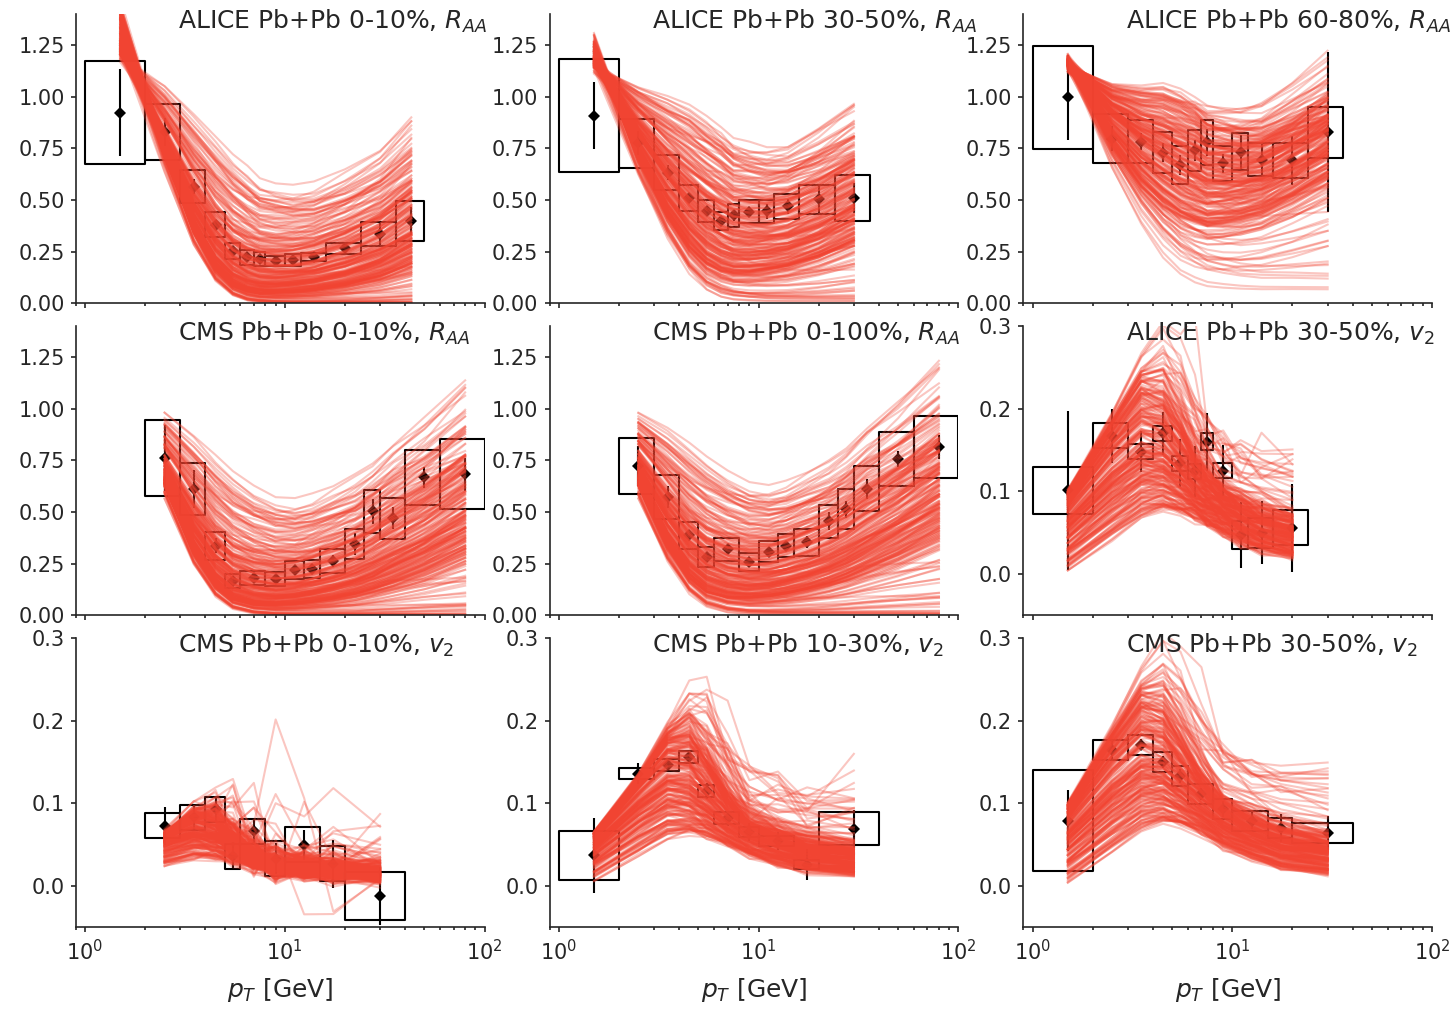
\includegraphics[width=\textwidth]{New-analysis/obs_prior.png}
\caption{•}
\label{fig:new:obs_prior}
\end{figure}

Computations of the model on both the design points and the validation points are performed on the NERSC super-computing system using over two million CPU hours.
The prior range of the observables are shown in figure \ref{fig:new:obs_prior}.
The $R_{AA}$ and $v_2$ of the heavy flavors are shown, with a good coverage of the data points.
Eight principal components are included, explaining 97.8\% of the data variance.
The validation is then performed on the 50 validation points.
We visualize the validation in figure \ref{fig:new:validation}.
In the top row, the emulated $v_2$ (left) and emulated $R_{AA}$ (right) are compared with the model calculations, and the data from different experiments and centrality has been labeled by different colors.
The emulated values strongly correlates with the true calculations around the the $y=x$ line.
Most points hit off the line, meaning the emulator has uncertainty.
To see if the emulator can reasonably estimate its uncertainty, in the bottom plots, we scatter plot the emulator's standard deviation ($\sigma$) of the prediction (the $y$ axis) versus the absolute value of the true deviation from between the prediction and the calculation (the $x$ axis).
The dashed line defines the shaded region where the true deviation is large than $\pm 3\sigma$.
We found that over $99\%$ of the $v_2$ and $R_{AA}$ points are within the $3\sigma$ region.
Therefore, for most cases the emulator correctly estimates its uncertainty and prevents an over interpretation.
For $v_2$ there is only a few outliers in outside of the three sigma region; for $R_{AA}$, there are more such points and shows certain systematic behavior.

\begin{figure}
\centering
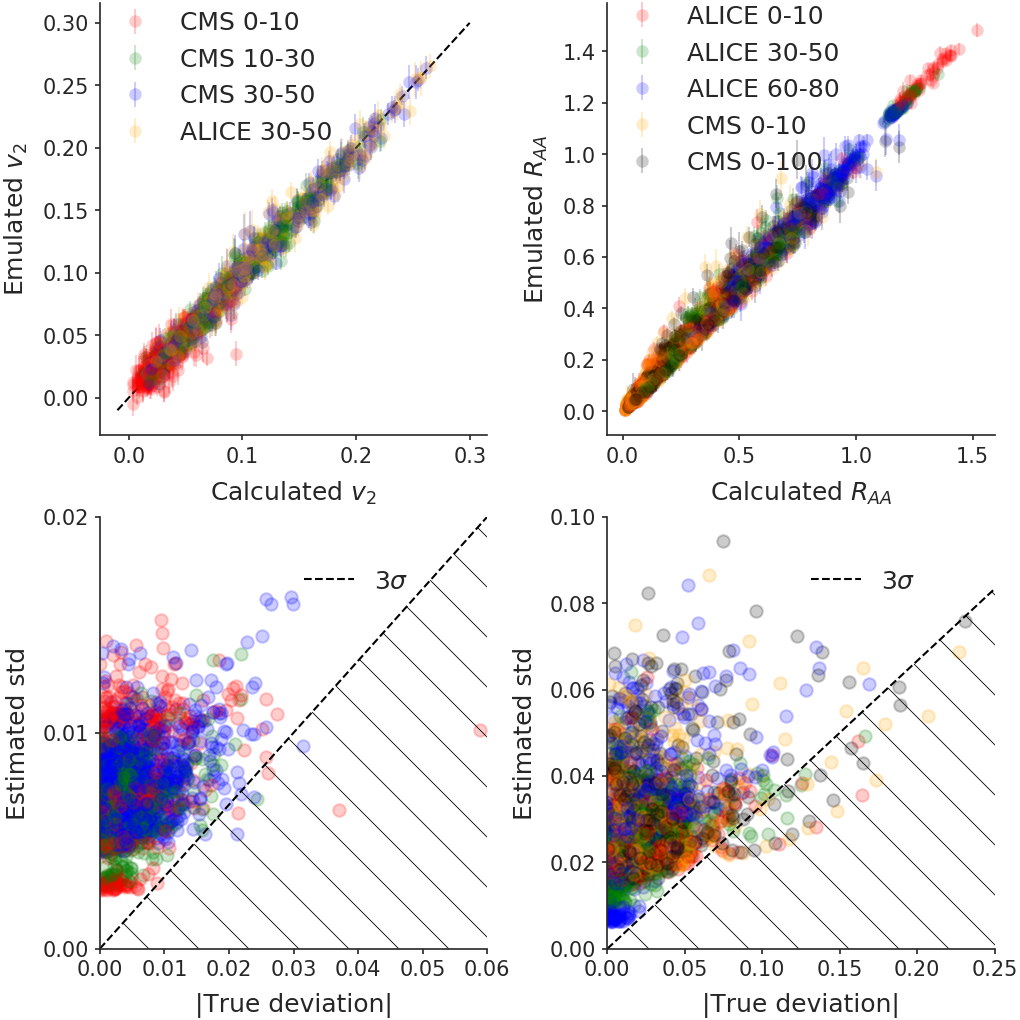
\includegraphics[width=\textwidth]{New-analysis/validation.png}
\caption{•}
\label{fig:new:validation}
\end{figure}

Now we specify the covariance matrix to define the likelihood function, and marginalize the posterior distribution function using the MCMC technique.
The general structure of the covariance matrix has been introduced in the previous section, here we use a centrality decorrelation factor $C=0.5$, and choses two different $\ln p_T$ correlation length $0.5$ and $1$ to how sensitive the calibration is to different form of covariance matrix.
We first take a look at the global level of agreement between the calibrated model and the data.
In figure 

\begin{figure}
\centering
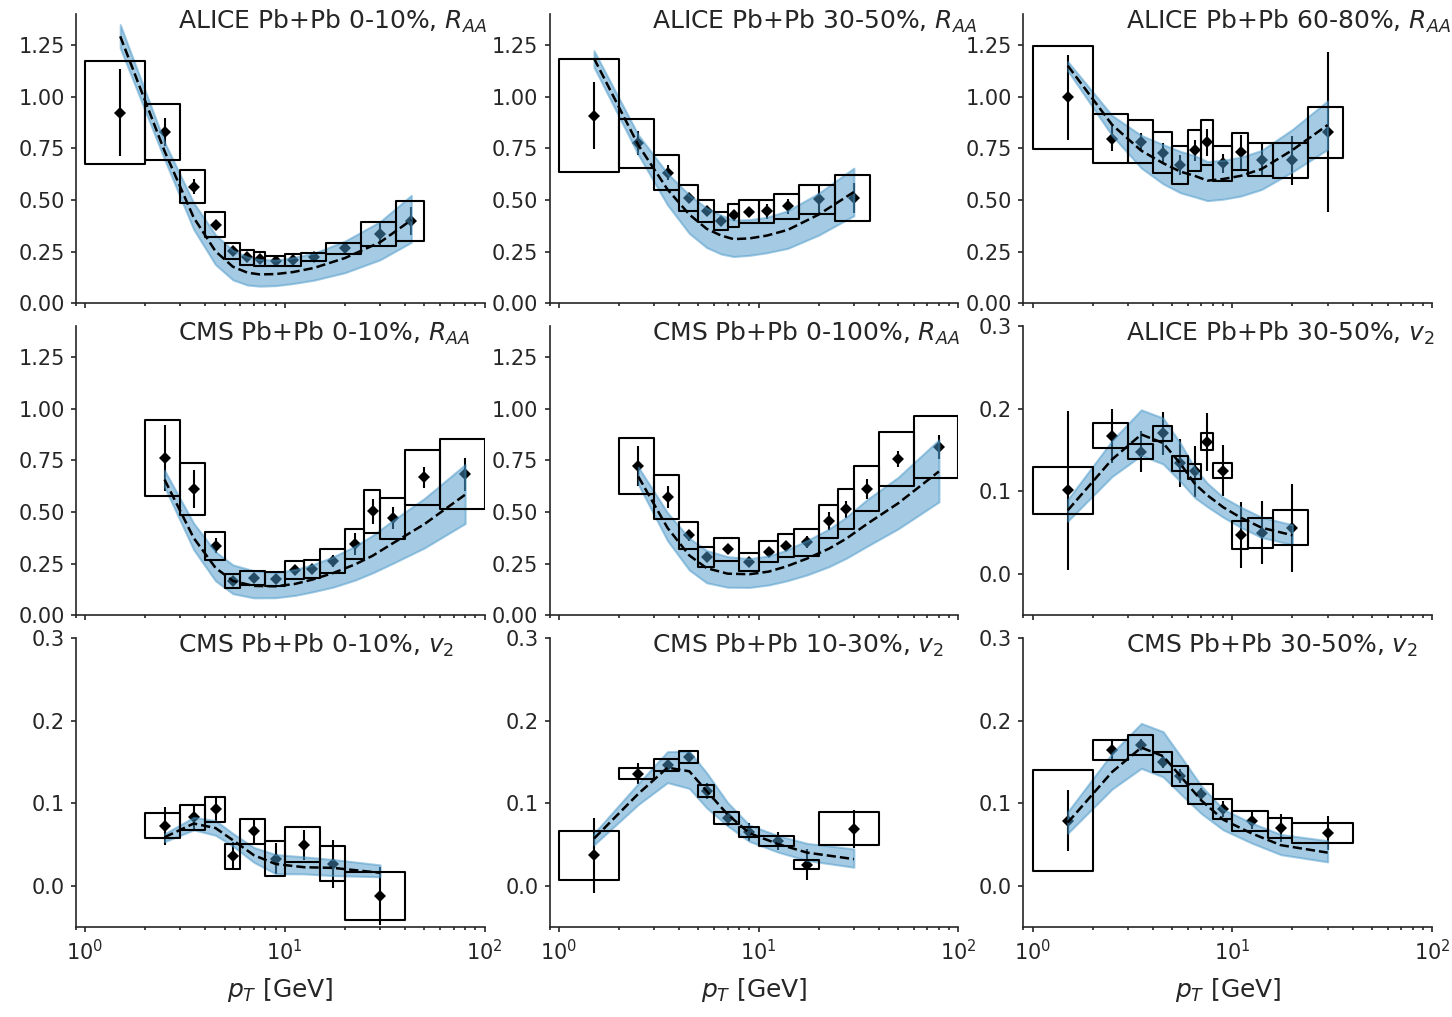
\includegraphics[width=\textwidth]{New-analysis/obs_posterior.png}
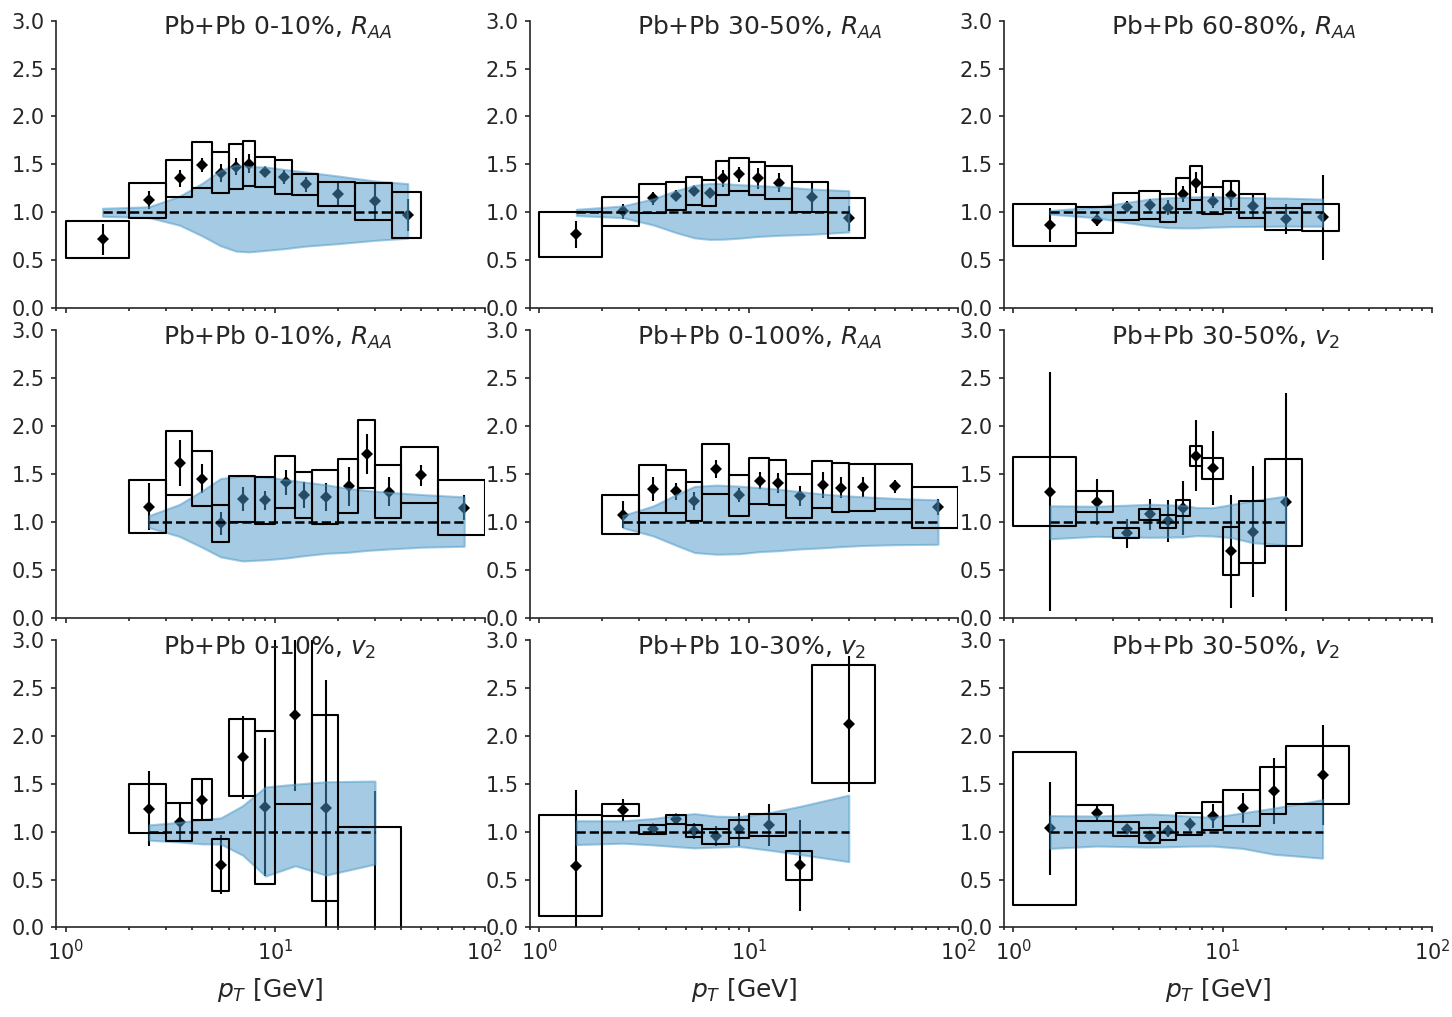
\includegraphics[width=.98\textwidth]{New-analysis/obs_ratio_posterior.png}
\caption{•}
\label{fig:new:obs_posterior}
\end{figure}

\begin{figure}
\centering
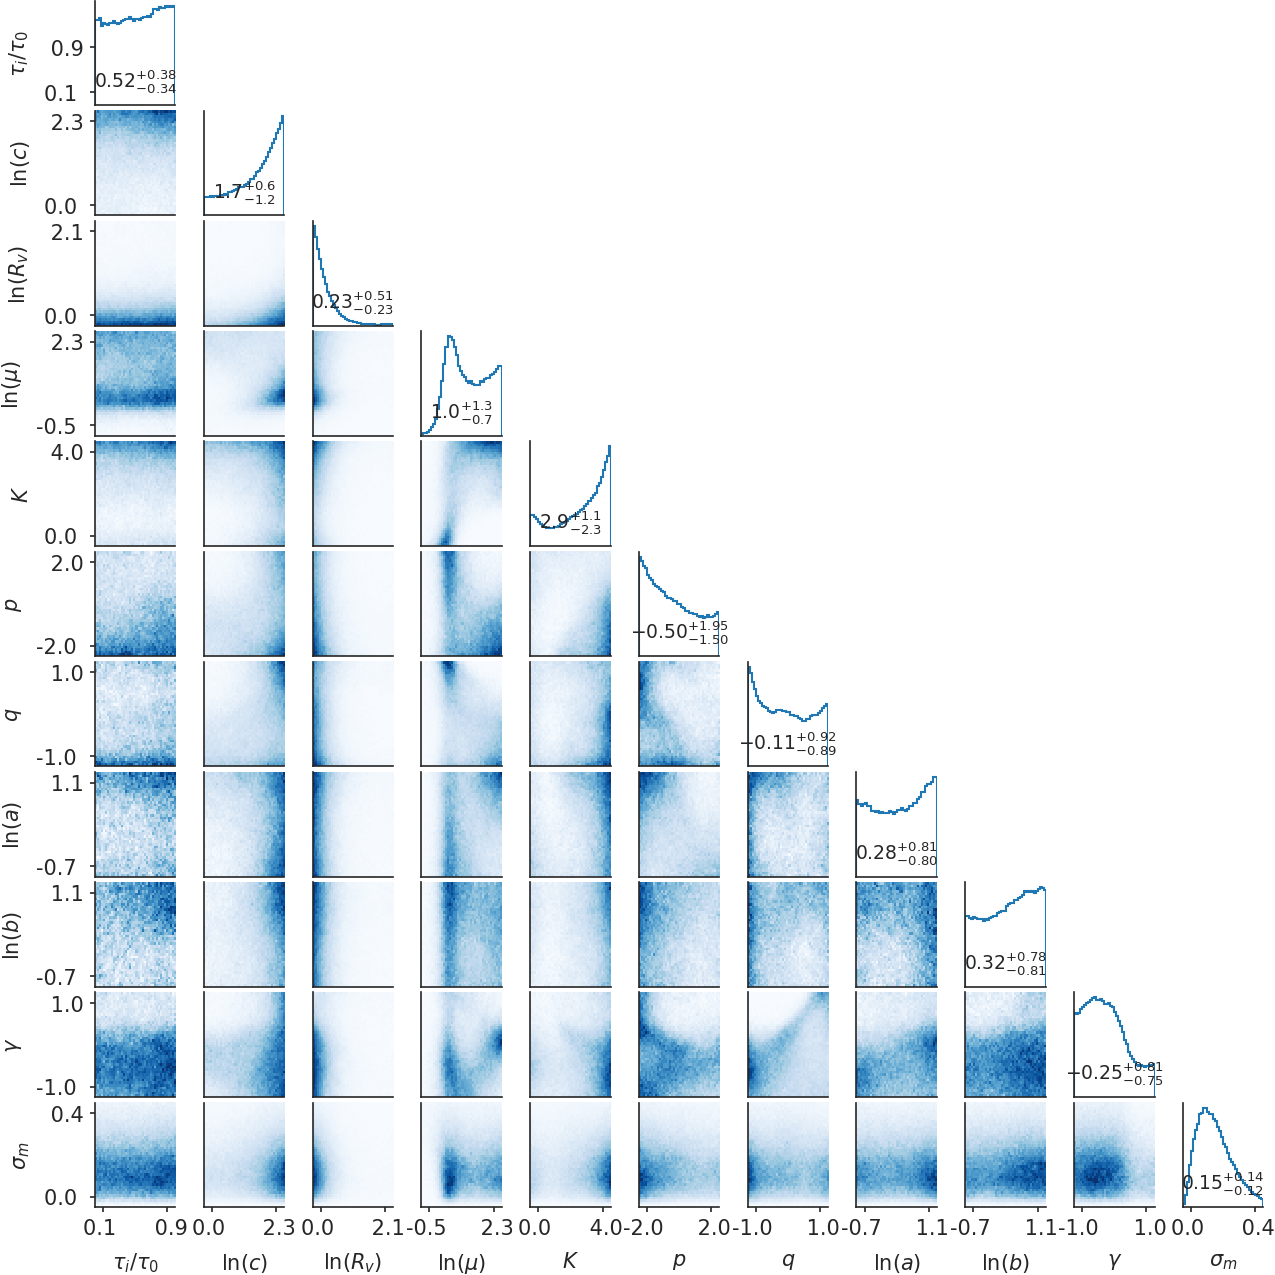
\includegraphics[width=\textwidth]{New-analysis/posterior-L0d3.png}
\caption{•}
\label{fig:new:posterior-l0d3}
\end{figure}

\begin{figure}
\centering
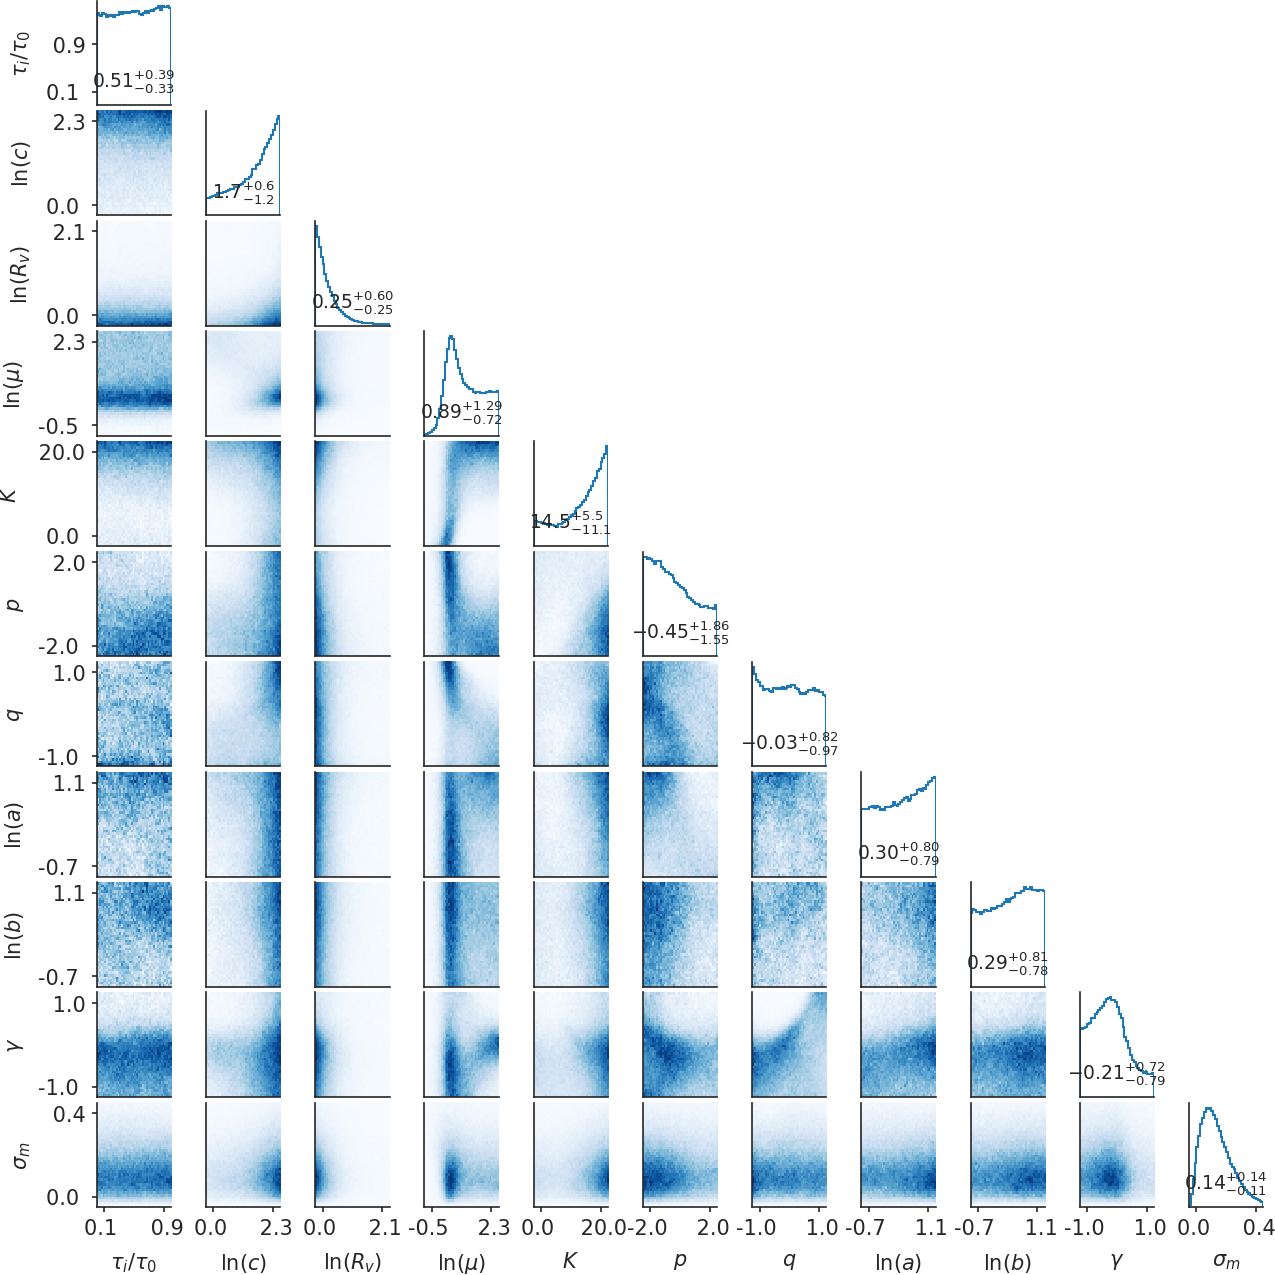
\includegraphics[width=\textwidth]{New-analysis/posterior-L0d5.png}
\caption{•}
\label{fig:new:posterior-l0d5}
\end{figure}

\begin{figure}
\centering
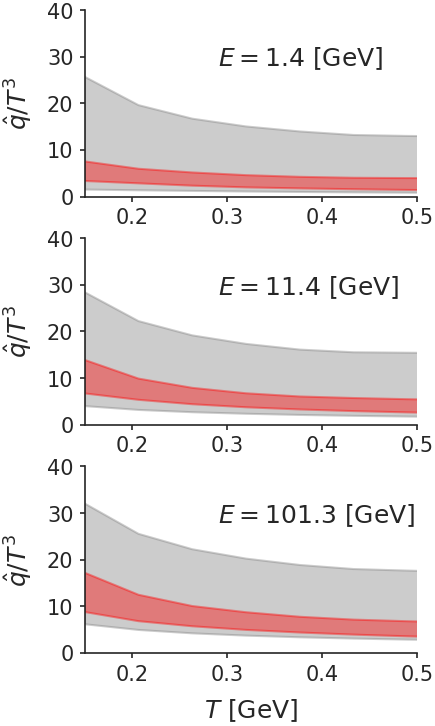
\includegraphics[width=.5\textwidth]{New-analysis/qhat_posterior.png}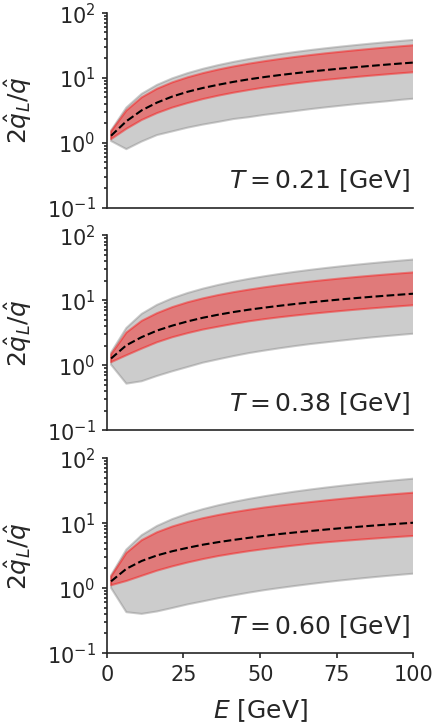
\includegraphics[width=.5\textwidth]{New-analysis/ER_posterior.png}
\caption{•}
\label{fig:new:posterior-qhat}
\end{figure}

\begin{figure}
\centering
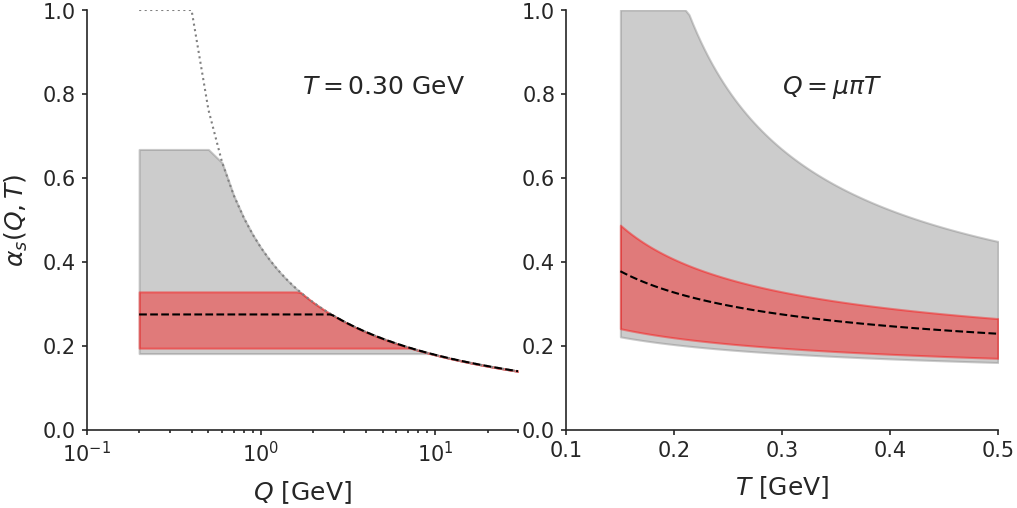
\includegraphics[width=.6\textwidth]{New-analysis/alpha_s_posterior.png}
\caption{•}
\label{fig:new:posterior-alphas}
\end{figure}
